\section{Experiment Condition}
The environment for the experiment is shown in Table \ref{tab:environment} and figure \ref{fig:home}, \ref{fig:servo}, \ref{fig:model}. Table \ref{tab:network} shows the expected network model.

\begin{table}[!h]
\begin{center}
\caption{experiment environment}
\label{tab:environment}
\begin{tabular}{|c|c|}
\hline
Operating System & Ubuntu14.04 LTS \\
\hline
Middleware & ROS indigo \\
\hline
Hardware & @home robot \\
\hline
Input Actuator & KONDO B3M-SC1170-A \\
\hline
Output Actuator & TF-M30-24-3500-G15R \\
\hline
Simulator & Gazebo 7.1 \\
\hline
\end{tabular}
\end{center}
\end{table}

\begin{table}[!h]
\begin{center}
\caption{network model}
\label{tab:network}
\begin{tabular}{|c|c|c|}
\hline
Layers & No. of Nodes & Activation \\
\hline
Input & 6 (joint error positions) & Linear \\
\hline
Hidden 1 & 100 & ReLU \\
\hline
Hidden 2 & 100 & ReLU \\
\hline
Output & 3 (forward, stop, reverse) &  \\
\hline
\end{tabular}
\end{center}
\end{table}

\begin{figure}[!h]
\begin{center}
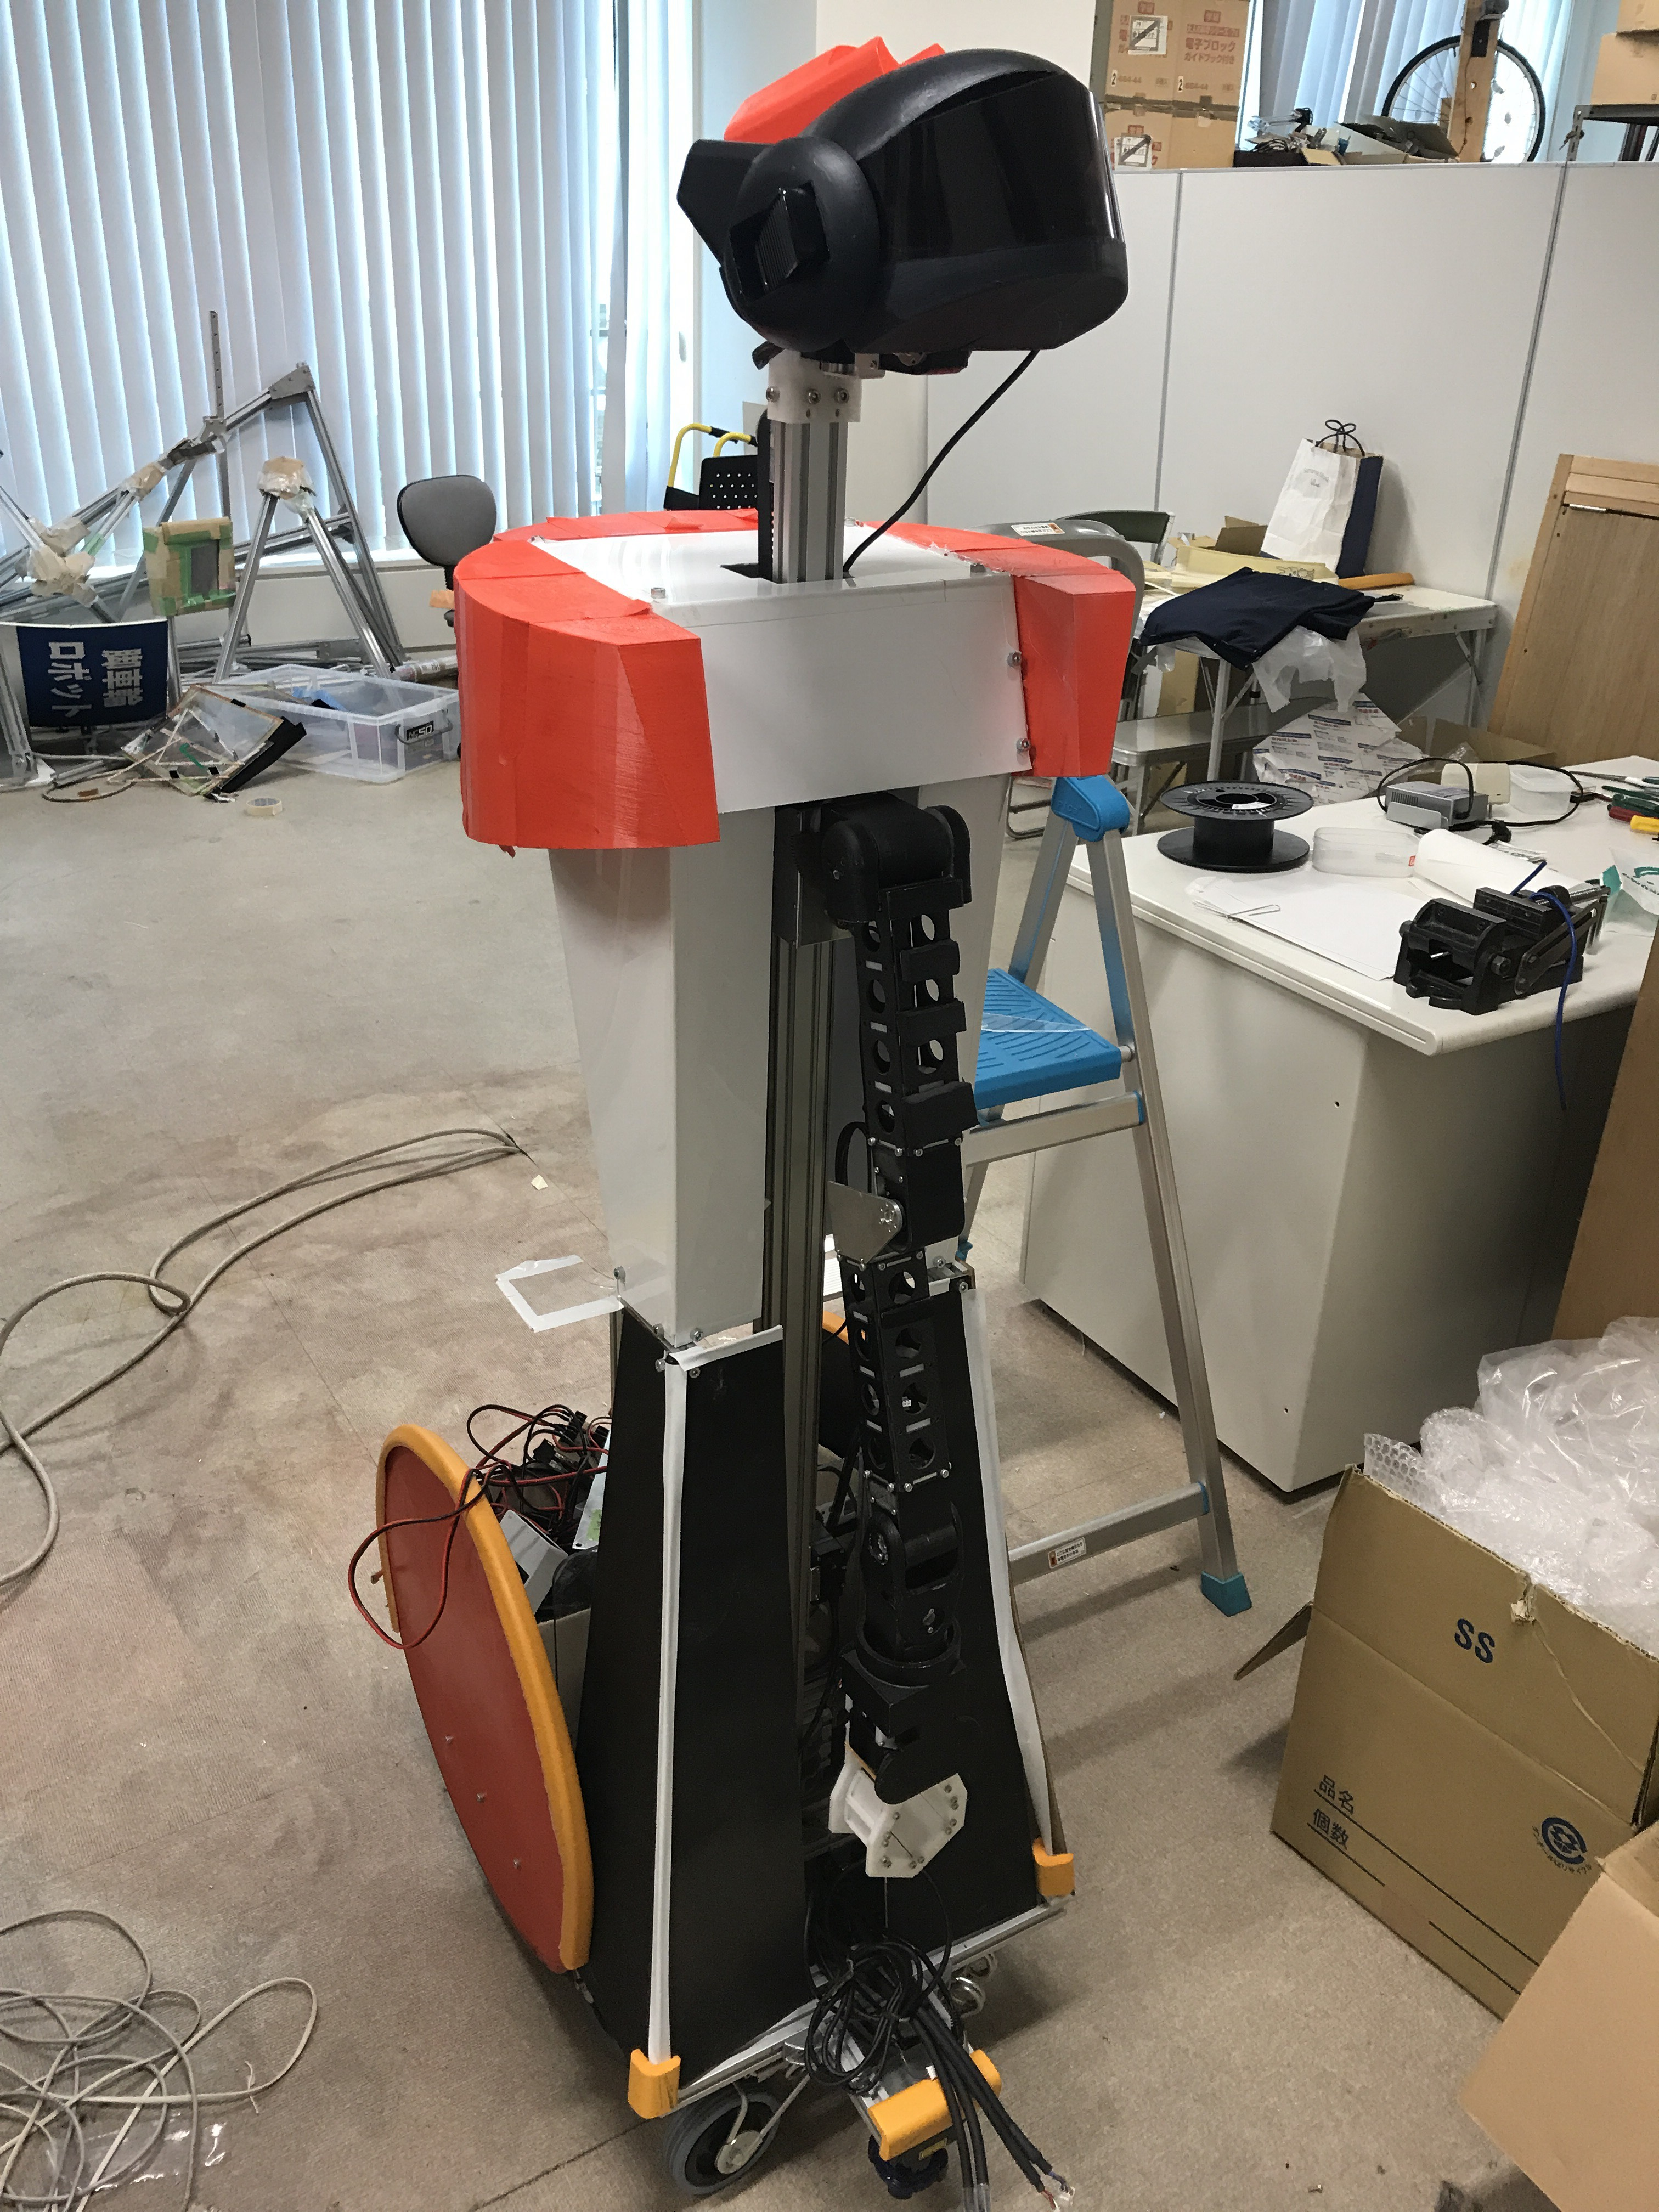
\includegraphics[width=5cm]{athome.jpg}
\caption{@home robot, hardware expected to use for this experiment}
\label{fig:home}
\end{center}
\end{figure}

\begin{figure}[!h]
\begin{center}
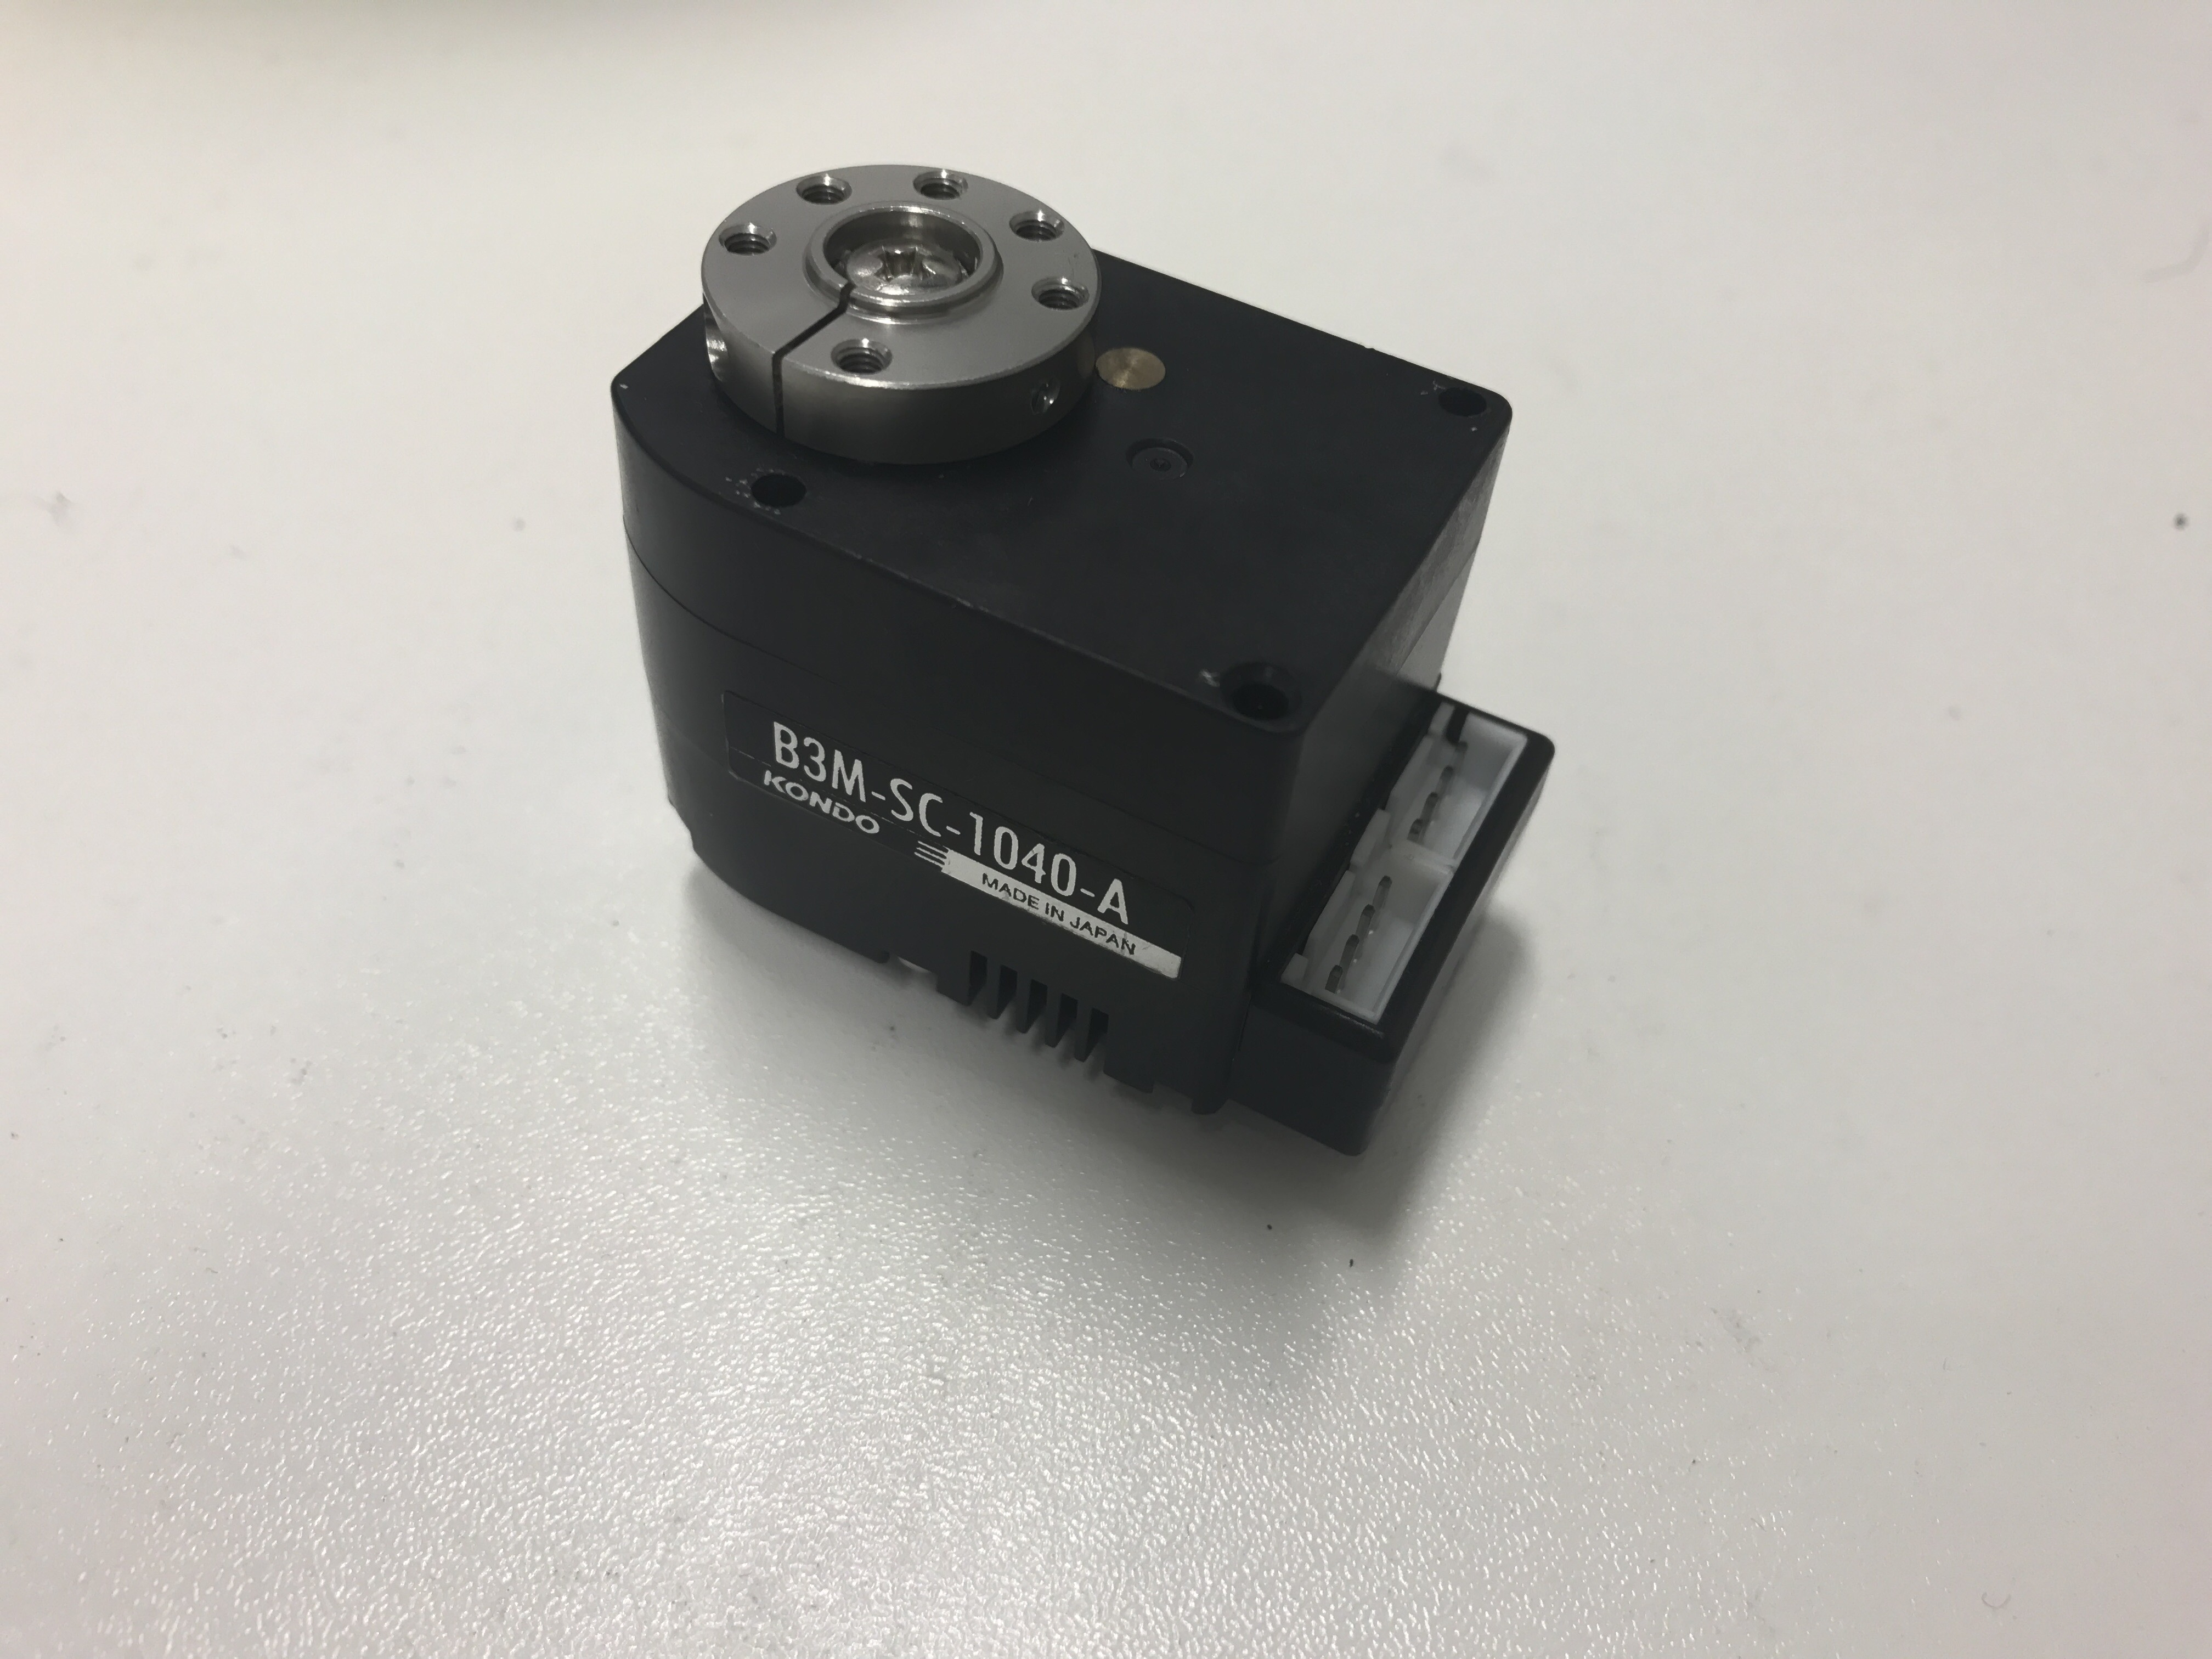
\includegraphics[width=5cm]{servo.jpg}
\caption{KONDO B3M-SC1170-A, input actuator used in manipulator}
\label{fig:servo}
\end{center}
\end{figure}

\begin{figure}[!h]
\begin{center}
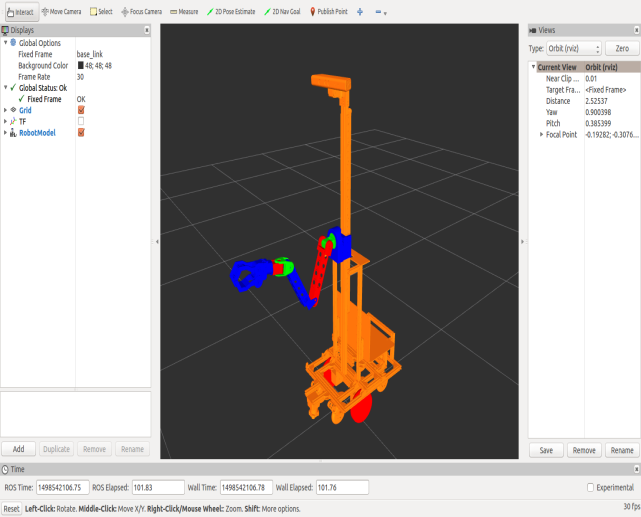
\includegraphics[width=5cm]{model.png}
\caption{robot model on simulator}
\label{fig:model}
\end{center}
\end{figure}